\section{Description and Methodology}

\subsection{Compiling the Linux kernel}
\begin{figure}[h]
	\centering
	
\includegraphics[width=3cm]{img/uclinux.png}
	\caption{uClinux logo}
	\label{fig:uclinux}
\end{figure}
We were supplied with a variant of Linux called \emph{uClinux}, and it's supplied toolchain. We built the distribution by using a build system named \emph{ptxdist}. We followed \cite[section 5.3]{compendium} step by step, and when done we ended up with a working linux distribuion on the chip, with Tux drawn on the screen. Initially we did not change the kernel config\footnote{We ended up doing so, please see section \ref{subsection:energy-efficiency}.}, nor add any more packages than already supplied and configured.

\subsection{Device driver for the gamepad}

\subsection{Signals and interrupts}
\label{subsection:signals-and-interrupts}
\subsubsection{Enabling and handling interrupts}
\emph{TODO sindre}

\subsubsection{Generating signals in kernel space}
\begin{figure}[h]
	\centering
	\lstinputlisting[frame=single, numbers=left]{code/signal_user_application.c}
	\caption{Signaling user space from kernel space}
	\label{fig:signal-user-application}
\end{figure}
The \vn{signal\_user\_application(void)} function in the \mn{driver-gamepad.c} sends a signal to the process who has the driver open. We have used the \textbf{SIGUSR1} signal, because it is documented to be set aside for you to use any way we want and is useful for interprocess communication. In addition to specifying signal type and process to receive the signal, we add the SI\_QUEUE to enable the signal to carry data from kernel to user space. See figure \ref{fig:signal-user-application}.

\subsubsection{Handle signals in user space}
\begin{figure}[h]
	\centering
	\lstinputlisting[frame=single, numbers=left]{code/sighandler.c}
	\caption{Adding signals handlers with signal mask to the user space}
	\label{fig:sighandler}
\end{figure}

\subsection{Controlling the screen}

\subsection{Pong}

\subsection{Driver concurrency}
When writing a driver, we need to handle concurrency in the utilization of the driver.
\paragraph{Only on handle allowed}
Using the \vn{device\_open} variable in \mn{driver-gamepad.c}, we made sure that only one handler of the driver could be open at any time. Because the open file operation is protected by a critical region in the Linux kernel, no race conditions can occur setting this variable.\\
\emph{TODO - Finne ut om det er riktig med kritisk region}
\paragraph{Signal mask}
As seen in lines 7-9 of figure \ref{fig:sighandler}, we set a signal mask when assigning signal handlers. By adding signals to this mask, we tell the operating system that these signals should be blocked while the signal handler is running. In this solution, the only code that modifies the game state is signal handlers for \textbf{SIGUSR1} (buttons) and \textbf{SIGALRM} (timer), and by adding these to the signal mask, we guarantee that the signal handlers will run one by one, making it impossible for race conditions and invalid program state.


\subsection{Energy efficiency}
\label{subsection:energy-efficiency}
As we are no longer programming on the "bare metal", we have less control over the software running on the chip. \emph{uClinux} have certain requirements regarding timers and other peripherals, and \cite{compendium} states that "all relevant clocks are already turned on", which we consider as a statement that says the oscilator setup is fixed, and should not be altered for this exercise. Still, we could use some techniques to reduce the energy consumption.

\subsubsection{Interrupts and signals}
We implemented our driver so no polling mechanisms were needed (as described in section \ref{subsection:signals-and-interrupts}). As a consequence, the program will stay most of its time in a \emph{pause()} loop, leaving the CPU and IO buses free to do other stuff, or in this case, sleep. This behaviour decreases power consumption.

\subsubsection{Optimizing screen update}
\emph{TODO sindre}

\subsubsection{Tickless idle}
\begin{figure}[h]
	\centering
	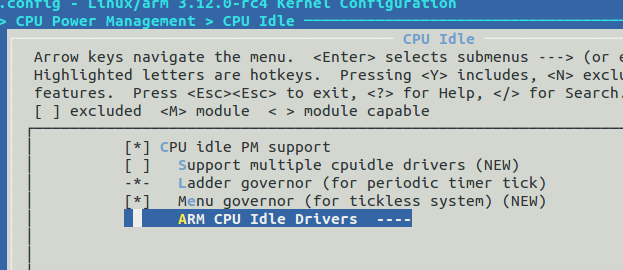
\includegraphics[width=12cm]{img/tickless.png}
	\caption{Configuring the kernel to tickless idle}
	\label{fig:tickless}
\end{figure}
Because our game is handeled entirely by signal handlers, leaving the main program in a pause loop, we wanted to reduce the power consumption while waiting for an interrupt/signal. In order to do that, we were adviced to put the kernel in a mode known as tickless idle. We did this by setting
